\section{Câu 2}
    \hspace*{0.6cm}\textbf{Chọn 1 vật bất kỳ. Tính toán tọa độ pixel và góc của vật}
    \subsection{Mục tiêu}

        \hspace*{0.6cm}Mục tiêu của bài thực hành là xây dựng một pipeline xử lý ảnh đơn giản để phát hiện một vật thể bất kỳ trong ảnh (trong thí nghiệm này là tấm card đặt trên nền tối), sau đó tính toán:

        \begin{itemize}
            \item Tọa độ pixel của trọng tâm vật thể (cx, cy).
            \item Góc xoay (orientation) của vật thể so với trục Ox của ảnh.
        \end{itemize}

    \subsection{Cơ sở lý thuyết:}

        \subsubsection{Hệ tọa độ ảnh}

            \hspace*{0.6cm}Trong OpenCV, hệ tọa độ ảnh được định nghĩa với gốc tọa độ tại góc trên bên trái của ảnh. Trục x tăng dần theo hướng từ trái sang phải, trục y tăng dần theo hướng từ trên xuống dưới. Một điểm ảnh bất kỳ được biểu diễn bởi cặp (u, v) hoặc (x, y) trong hệ tọa độ này.

        \subsubsection{Moment và trọng tâm hình dạng}

            \hspace*{0.6cm}Với một vùng liên thông bất kỳ trong ảnh nhị phân, có thể sử dụng moment hình học để tính trọng tâm. OpenCV cung cấp hàm cv2.moments() cho contour, trả về các moment $m_{ij}$. Trọng tâm (cx, cy) được tính theo công thức:

            \begin{equation}
                cx = \frac{m_{10}}{m_{00}}
            \end{equation}

            \begin{equation}
                cy = \frac{m_{01}}{m_{00}}
            \end{equation}

            Với:
            \begin{itemize}

                \item $m_{00}$ được gọi là moment bậc 0, moment này chính là diện tích của đối tượng.

                \item $m_{10}$ hay $m_{01}$ được gọi là moment bậc nhất, chứa thông tin về vị trí tâm của vật.
            \end{itemize}
        \subsubsection{Contour và hình chữ nhật bao xoay}

            \hspace*{0.6cm}Contour là đường biên khép kín mô tả ranh giới của một vùng trong ảnh nhị phân. Hàm cv2.findContours() được sử dụng để trích xuất các contour từ ảnh nhị phân. Để mô tả hướng của vật thể, ta sử dụng hàm cv2.minAreaRect(), hàm này tìm hình chữ nhật có diện tích nhỏ nhất bao trọn contour (minimum area bounding rectangle). Kết quả trả về gồm:

            \begin{itemize}
                \item Tọa độ tâm hình chữ nhật.
                \item Góc quay của hình chữ nhật so với trục Ox theo quy ước của OpenCV.
            \end{itemize}

            Từ bốn đỉnh của hình chữ nhật bao xoay, ta có thể xác định các cạnh và chọn cạnh dài nhất làm phương của vật thể (ví dụ cạnh dài của tấm card).

            \begin{itemize}
                \item Dựa trên vector của cạnh này, có thể tính góc xoay bằng hàm $atan2: angle = atan2(dy, dx)$, sau đó đổi sang đơn vị độ.
            \end{itemize}

    \subsection{Các bước thực hiện}

        \subsubsection{Bước 1 – Đọc ảnh và tiền xử lý}

            \hspace*{0.6cm}Ảnh màu được đọc bằng cv2.imread() và lưu thêm một bản sao để vẽ kết quả. Sau đó, ảnh được chuyển sang ảnh xám bằng cv2.cvtColor() và làm mờ Gaussian nhằm giảm nhiễu cục bộ, giúp bước nhi phân hóa ổn định hơn.

        \subsubsection{Bước 2 – Nhi phân hóa và lọc nhiễu}

            \hspace*{0.6cm}Vì tấm card sáng hơn so với nền đen nên sử dụng phương pháp phân ngưỡng Otsu với kiểu cv2.THRESH\_BINARY. Phương pháp Otsu tự động chọn ngưỡng tối ưu dựa trên histogram của ảnh xám. Sau khi nhi phân hóa, ảnh được áp dụng phép toán hình thái học: mở (opening) để loại bỏ các điểm nhiễu nhỏ và đóng (closing) để lấp các lỗ nhỏ bên trong vùng card. Kết quả thu được ảnh nhi phân sạch, trong đó card là một khối liên thông trắng trên nền đen.

        \subsubsection{Bước 3 – Tìm contour của vật thể}

            \hspace*{0.6cm}Hàm cv2.findContours() với chế độ RETR\_EXTERNAL được sử dụng để chỉ lấy các contour ngoài cùng. Từ danh sách các contour, chương trình chọn contour có diện tích lớn nhất (max theo cv2.contourArea()), giả sử đó là contour của tấm card vì card là đối tượng sáng lớn nhất trên ảnh.

        \subsubsection{Bước 4 – Tính trọng tâm vật thể}

            \hspace*{0.6cm}Sau khi xác định contour lớn nhất, chương trình gọi cv2.moments() để tính các moment hình học. Trọng tâm (cx, cy) của card được tính bằng công thức:

            \begin{equation}
                cx = \frac{m_{10}}{m_{00}}, cy = \frac{m_{01}}{m_{00}}
            \end{equation}

            Kết quả là tọa độ pixel của trọng tâm card trong hệ tọa độ ảnh.

        \subsubsection{Bước 5 – Tính góc xoay của vật thể}

            \hspace*{0.6cm}Để xác định hướng của card, chương trình sử dụng cv2.minAreaRect() trên contour lớn nhất. Hàm này trả về một hình chữ nhật xoay. Từ bốn đỉnh của hình chữ nhật, ta lần lượt xét bốn cạnh và tình cạnh có độ dài lớn nhất được coi là hướng chính (cạnh dài) của vật thể. Góc xoay tương ứng được tính bằng:

            \begin{equation}
                angle_{rad} = atan2(dy, dx) \rightarrow angle_{deg} = angle_{rad} \times \frac{180}{\pi}
            \end{equation}

            Sau đó, góc được chuẩn hóa về khoảng $(-90°, 90°]$ để thuận tiện cho việc hiển thị và so sánh.

        \subsubsection{Bước 6 – Hiển thị và lưu kết quả}

            \hspace*{0.6cm}Cuối cùng, chương trình vẽ contour của card, hình chữ nhật bao xoay, trọng tâm (dấu chấm màu) và thước đo (dòng chữ) thể hiện tọa độ trọng tâm cùng góc xoay lên bản sao ảnh gốc được hiển thị bằng cv2.imshow() và đồng thời lưu lại dưới dạng file PNG để phục vụ việc báo cáo và đánh giá.

    \subsection{Thực nghiệm và kết quả}
        \hspace*{0.6cm}Ảnh đầu vào: ảnh chụp tấm card visit trên nền đen.
        \begin{figure}[H]
            \centering
            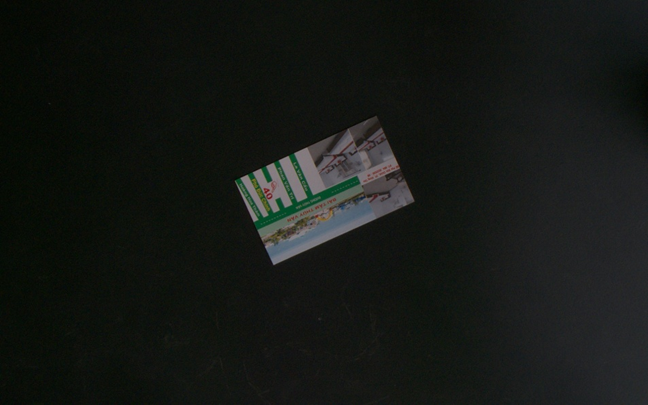
\includegraphics[width=0.8\textwidth]{pictures/section2/s2_p01.png}
            \caption{Ảnh đầu vào}
            \label{fig:working_distance}
        \end{figure}
        \textbf{Kết quả thu được từ code:}
        \begin{figure}[H]
            \centering
            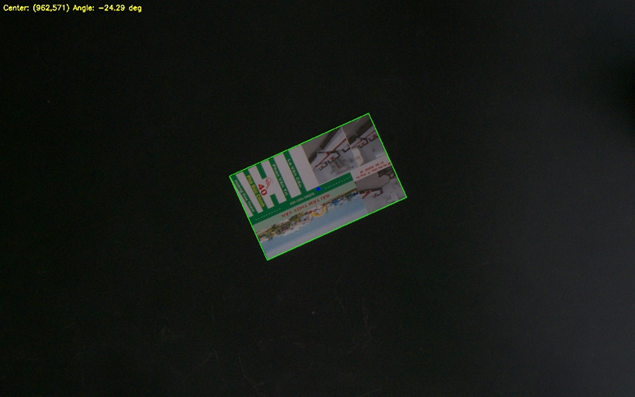
\includegraphics[width=0.8\textwidth]{pictures/section2/s2_p02.png}
            \caption{Kết quả sau khi chạy chương trình kèm thông tin tọa độ và góc xoay}
            \label{fig:working_distance}
        \end{figure}

        Khi chạy chương trình trên ảnh, ta thu được kết quả in trên ảnh như sau:

        \begin{itemize}
            \item Tọa độ trọng tâm card: $Center \approx (962, 571) pixel$.
            \item Góc xoay của card: $Angle \approx -24.29°$.
        \end{itemize}

        Giá trị góc âm thể hiện rằng card nghiêng theo một hướng nhất định so với trục Ox trong hệ tọa độ ảnh (trong ví dụ này, y hướng xuống). Góc xoay thu được phù hợp với quan sát trực quan trên ảnh: card quay ngược chiều so với phương ngang một góc khoảng 24°.

        \textbf{Kết quả từ tính toán trên paint và đo góc:}
        \begin{figure}[H]
            \centering
            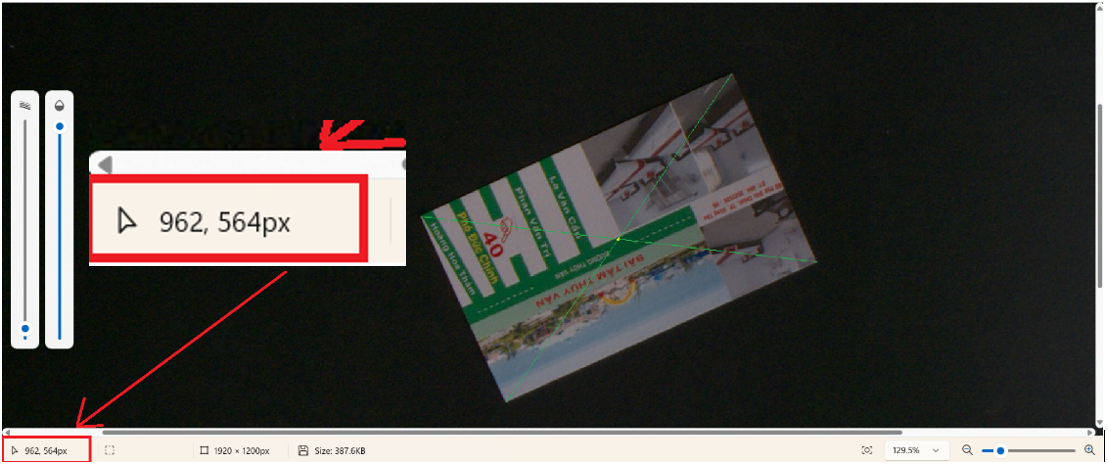
\includegraphics[width=1\textwidth]{pictures/section2/s2_p03.png}
            \caption{Hình ảnh thể hiện tọa độ tâm pixel}
            \label{fig:working_distance}
        \end{figure}
        \begin{figure}[H]
            \centering
            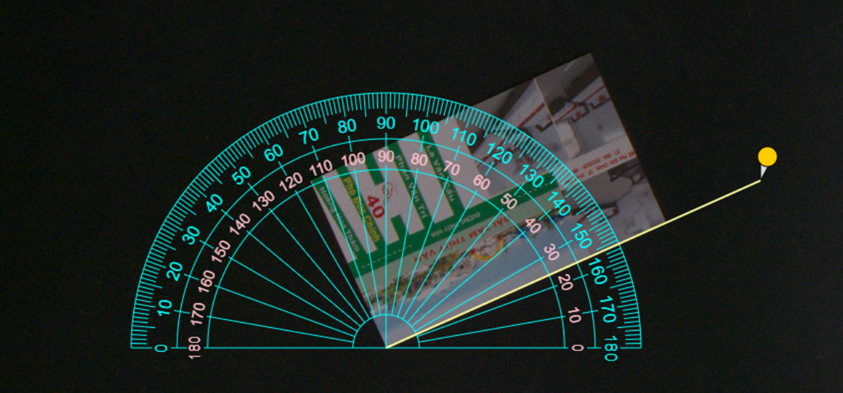
\includegraphics[width=1\textwidth]{pictures/section2/s2_p04.png}
            \caption{Hình ảnh thể hiện góc xoay của vật}
            \label{fig:working_distance}
        \end{figure}
